\section{Auswertung}
\label{sec:Auswertung}

\subsection{Zählrohr-Charakteristik}
\begin{table*} [h]
  \centering
  \caption{Messwerte Geiger-Müller-Charakteristik}
  \label{tab:Messdaten Geiger-Mueller-Charakteristik}
  \begin{tabular}{cccccc}
  \toprule
  $U\,[V]$ & $N\,[Imp/60s]$ &  $I\,[\mu A]$ &&  $U\,[V]$ & $N\,[Imp/60s]$ &  $I\,[\mu A]$\\
  \midrule
  320 & 9672 & && 520 & 10255 & \\
  330 & 9689 & && 530 & 10151 & \\
  340 & 9580 & 0.3 && 550 & 10184 & 1.0\\
  360 & 9886  &  && 560 & 10137 & \\
  370 & 10041 &  && 570 & 10186 & \\
  380 & 9996  &  && 580 & 10171 & \\
  390 & 9943  &  && 590 & 10171 & \\
  400 & 9995  & 0.4 && 600 & 10253 & 1.3\\
  410 & 9980  &  && 610 & 10368 & \\
  420 & 9986  &  && 620 & 10365 & \\
  430 & 9960  &  && 630 & 10224 & \\
  440 & 10219 &  && 640 & 10338 & \\
  450 & 10264 &  0.7 && 650 & 10493 & 1.4\\
  460 & 10174 &  && 660 & 10467 & \\
  470 & 10035 &  && 670 & 10640 & \\
  480 & 10350 &  && 680 & 10939 & \\
  490 & 10290 &  && 690 & 11159 & \\
  500 & 10151 &  0.8 && 700 & 11547 & 1.8\\
  510 & 10110 & && & & \\
    \bottomrule
\end{tabular}
\end{table*}

\subsection{ zeitlichen Abstand zwischen Primär- und Nachentladungsimpulsen}


\subsection{Bestimmung de Totzeit}
Mit dem Oszilloskop:\\
Mit der Zwei-Quellen-Methode:\\
\begin{align*}
  N_1 = 96041 Imp/120s\\
  N_{1+2} = 158579 Imp/120s\\
  N_2 = 76518 Imp/120s.
\end{align*}

\subsection{Bestimmung des Zählrohrstroms}
\begin{table*} [h]
  \centering
  \caption{Messwerte Zählerstrom}
  \label{tab:Messdaten Zaehlerstrom}
  \begin{tabular}{cc}
  \toprule
    U [V] & I [mu A]\\
    \midrule
    350 & 0.3\\
    400	& 0.4\\
    450	& 0.7\\
    500	& 0.8\\
    550	& 1.0\\
    600	& 1.3\\
    650	& 1.4\\
    700	& 1.8\\
    \bottomrule
  \end{tabular}
  \end{table*}
%\begin{figure}
  %\centering
  %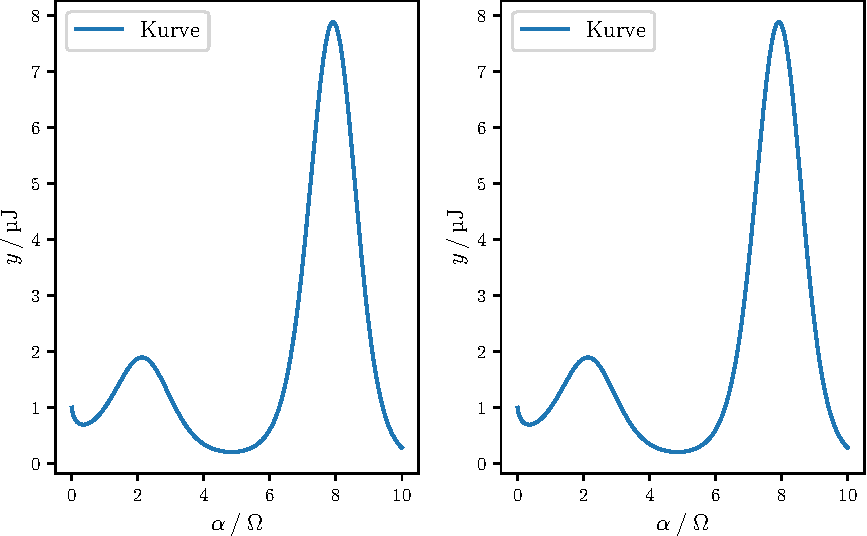
\includegraphics{plot.pdf}
  %\caption{Plot.}
  %\label{fig:plot}
%\end{figure}


%Siehe \autoref{fig:plot}!
